\documentclass[12pt]{article}
\usepackage{amsmath}
\usepackage{graphicx}
\usepackage{hyperref}
\usepackage{listings}
\usepackage{color}
\usepackage{pythonhighlight}

\title{Operating System Course Report - First Half of the Semester}
\author{B class}
\date{\today}

\begin{document}

\maketitle
\newpage

\tableofcontents
\newpage

\section{Introduction}
This report summarizes the topics covered during the first half of the Operating System course. It includes theoretical concepts, practical implementations, and assignments. The course focuses on the fundamentals of operating systems, including system architecture, process management, CPU scheduling, and deadlock handling.

\section{Course Overview}
\subsection{Objectives}
The main objectives of this course are:
\begin{itemize}
    \item To understand the basic components and architecture of a computer system.
    \item To learn process management, scheduling, and inter-process communication.
    \item To explore file systems, input/output management, and virtualization.
    \item To study the prevention and handling of deadlocks in operating systems.
\end{itemize}

\subsection{Course Structure}
The course is divided into two halves. This report focuses on the first half, which covers:
\begin{itemize}
    \item Basic Concepts and Components of Computer Systems
    \item System Performance and Metrics
    \item System Architecture of Computer Systems
    \item Process Description and Control
    \item Scheduling Algorithms
    \item Process Creation and Termination
    \item Introduction to Threads
    \item File Systems
    \item Input and Output Management
    \item Deadlock Introduction and Prevention
    \item User Interface Management
    \item Virtualization in Operating Systems
\end{itemize}

\section{Topics Covered}

\subsection{Basic Concepts and Components of Computer Systems}
This section explains the fundamental components that make up a computer system, including the CPU, memory, storage, and input/output devices.

\subsection{System Performance and Metrics}
This section introduces various system performance metrics used to measure the efficiency of a computer system, including throughput, response time, and utilization.

\subsection{System Architecture of Computer Systems}
Describes the architecture of modern computer systems, focusing on the interaction between hardware and the operating system.

\subsection{Process Description and Control}
Processes are a central concept in operating systems. This section covers:
\begin{itemize}
    \item Process states and state transitions
    \item Process control block (PCB)
    \item Context switching
\end{itemize}

\subsection{Scheduling Algorithms}
This section covers:
\begin{itemize}
    \item First-Come, First-Served (FCFS)
    \item Shortest Job Next (SJN)
    \item Round Robin (RR)
\end{itemize}
It explains how these algorithms are used to allocate CPU time to processes.

\subsection{Process Creation and Termination}
Details how processes are created and terminated by the operating system, including:
\begin{itemize}
    \item Process spawning
    \item Process termination conditions
\end{itemize}

\subsection{Introduction to Threads}
This section introduces the concept of threads and their relation to processes, covering:
\begin{itemize}
    \item Single-threaded vs. multi-threaded processes
    \item Benefits of multithreading
\end{itemize}

\begin{figure}[h]
    \centering
    \includegraphics[width=0.5\textwidth]{/Users/khawaritzmi/Unhas/os_report_mid2024/b_class/asset/example.png}  % Sesuaikan nama file dan ukurannya
    \caption{Ini adalah gambar contoh dari multithreading.}
    \label{fig:contoh_gambar}
\end{figure}

Seperti yang terlihat pada Gambar \ref{fig:contoh_gambar}, inilah cara menambahkan gambar dengan keterangan.

\subsection{File Systems}
File systems provide a way for the operating system to store, retrieve, and manage data. This section explains:
\begin{itemize}
    \item File system structure
    \item File access methods
    \item Directory management
\end{itemize}

\subsection{Input and Output Management}
Input and output management is key for handling the interaction between the system and external devices. This section includes:
\begin{itemize}
    \item Device drivers
    \item I/O scheduling
\end{itemize}

\subsection{Deadlock Introduction and Prevention}
Explores the concept of deadlocks and methods for preventing them:
\begin{itemize}
    \item Deadlock conditions
    \subsection{Pencegahan Deadlock}
Pencegahan deadlock adalah usaha untuk mencegah terjadinya kondisi deadlock dengan cara menghindari salah satu dari empat faktor penyebab deadlock:

\begin{itemize}
    \item \textbf{Mutual Exclusion}: 
    Membuat sumber daya dapat dibagi (\textit{shared}) jika memungkinkan, sehingga lebih dari satu proses dapat mengaksesnya pada saat bersamaan.
    
    \item \textbf{Hold and Wait}: 
    Mencegah proses menahan sumber daya sambil menunggu sumber daya lain. Proses harus meminta semua sumber daya yang dibutuhkan di awal, atau melepaskan semua sumber daya sebelum meminta yang lain.
    
    \item \textbf{No Preemption}: 
    Mengizinkan sumber daya untuk diambil secara paksa dari suatu proses jika proses tersebut sedang menunggu sumber daya lain, untuk mencegah penahanan sumber daya terlalu lama.
    
    \item \textbf{Circular Wait}: 
    Mencegah siklus dalam permintaan sumber daya dengan memberikan nomor atau urutan pada sumber daya dan memastikan proses harus meminta sumber daya sesuai urutan tersebut.
\end{itemize}

\subsection{Faktor Penyebab Deadlock}
Empat faktor utama yang menyebabkan terjadinya deadlock adalah sebagai berikut:

\begin{itemize}
    \item \textbf{Mutual Exclusion}:
    Mutual Exclusion adalah kondisi di mana sumber daya hanya dapat diakses oleh satu proses pada satu waktu. Tiga syarat utama yang harus dipenuhi:
    \begin{itemize}
        \item Satu proses di \textit{critical region}: Hanya satu proses yang diperbolehkan berada dalam \textit{critical region} pada satu waktu. \textit{Critical region} adalah bagian dari program di mana akses eksklusif ke sumber daya dibutuhkan.
        \item Proses di luar \textit{critical region} tidak mengganggu: Proses yang berada di luar \textit{critical region} tidak boleh menghalangi atau memengaruhi proses lain yang ingin masuk ke \textit{critical region}.
        \item Akses adil ke \textit{critical region}: Tidak ada proses yang dicegah atau ditolak terus-menerus untuk masuk ke \textit{critical region}.
          \begin{figure}[htbp]
    \centering
    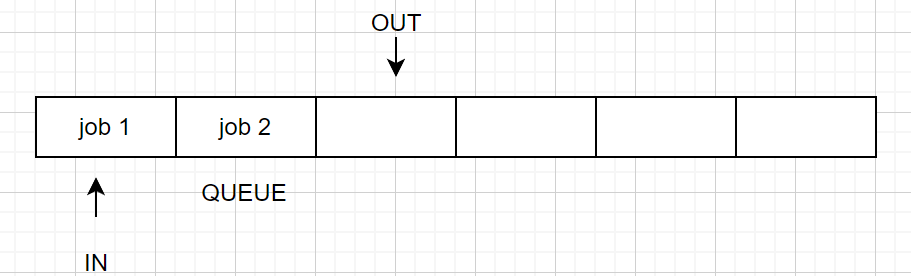
\includegraphics[width=1\linewidth]{asset/Mutual exclusion.png}
    \caption{MUTUAL EXCLUSION}
    \label{fig:enter-label}
    \end{figure}
    \end{itemize}
    
    \item \textbf{No Preemption}:
    \textit{Non-preemptive resource allocation} adalah kondisi di mana sumber daya hanya dapat dibebaskan secara sukarela oleh proses yang memilikinya. Proses tidak dapat dipaksa untuk melepaskan sumber daya yang sedang digunakan. Jika suatu proses meminta sumber daya tambahan yang tidak tersedia, semua sumber daya yang dipegang akan dilepaskan dan proses tersebut akan ditambahkan ke daftar tunggu.

    \begin{figure}
        \centering
        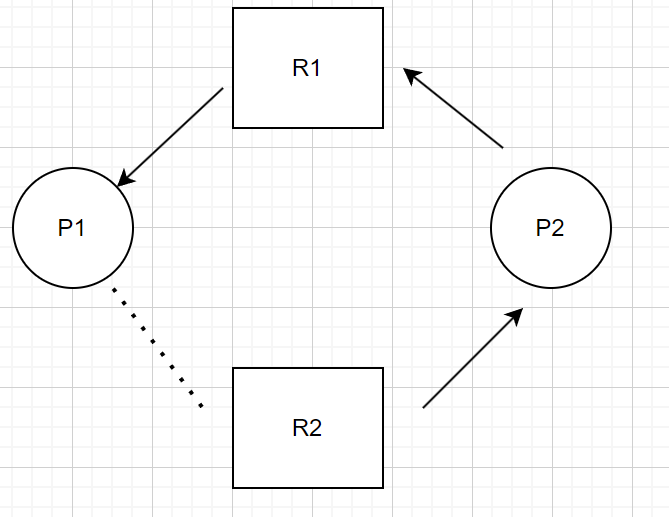
\includegraphics[width=0.5\linewidth]{asset/no preemption.png}
        \caption{NO PREEMPTION}
        \label{fig:enter-label}
    \end{figure}

    \item \textbf{Circular Waiting}:
    \textit{Circular Waiting} terjadi ketika proses-proses saling menunggu sumber daya yang dipegang oleh proses lain, sehingga membentuk rantai tunggu (\textit{waiting chain}). Untuk mencegah kondisi ini, setiap sumber daya diberi prioritas atau urutan, dan proses hanya dapat meminta sumber daya sesuai urutan prioritas yang meningkat.

   \begin{figure}
       \centering
       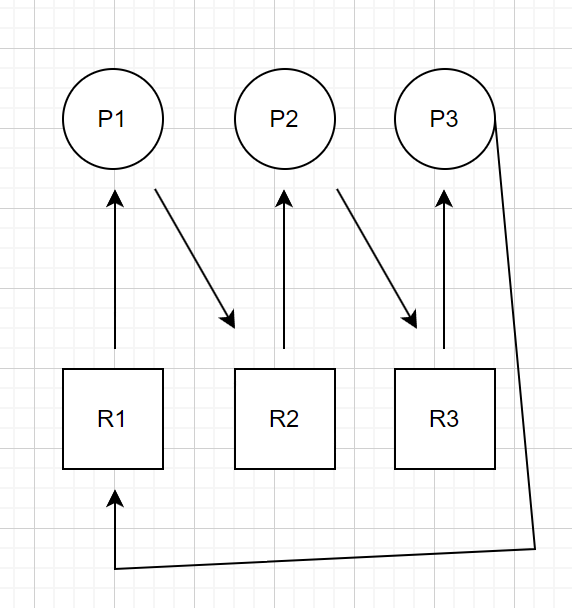
\includegraphics[width=0.25\linewidth]{asset/circular waiting.png}
       \caption{CIRCULAR WAITING}
       \label{fig:enter-label}
   \end{figure}
    
    \item \textbf{Hold and Wait}:
    \textit{Hold and Wait} adalah kondisi di mana suatu proses menahan satu sumber daya dan menunggu sumber daya lain. Untuk menghindari kondisi ini, ada beberapa pendekatan:
    \begin{itemize}

    \begin{figure}
        \centering
        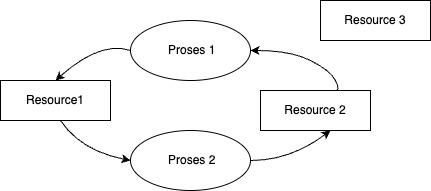
\includegraphics[width=0.5\linewidth]{asset/hold and wait.jpg}
        \caption{HOLD AND WAIT}
        \label{fig:enter-label}
    \end{figure}

        \item Menghilangkan penantian (\textit{Eliminating Wait}): Proses harus meminta semua sumber daya yang diperlukan sebelum eksekusi dimulai.
        \item Menghilangkan penahanan (\textit{Eliminating Hold}): Proses harus melepaskan semua sumber daya yang sedang dipegang sebelum meminta sumber daya baru.

\end{itemize}
    \end{itemize}
\end{itemize}

\textbf{Contoh Situasi}:
\begin{itemize}
    \item \textit{Resource 1} dialokasikan ke Proses 2.
    \item \textit{Resource 2} dan \textit{Resource 3} dialokasikan ke Proses 1.
    \item Proses 1 menunggu \textit{Resource 1} dan menahan \textit{Resource 2} dan \textit{Resource 3}.
    \item Proses 2 menunggu \textit{Resource 2} dan menahan \textit{Resource 1}.

    \begin{thebibliography}{9}

\bibitem{zflas} 
ZFLAS. 
\textit{Pengertian Deadlock: Penjelasan Lengkap Tentang Situasi Kebuntuan di Dunia Komputasi}. 
Diakses dari: \url{https://zflas.co/id/848/pengertian-deadlock-penjelasan-lengkap-tentang-situasi-kebuntuan-di-dunia-komputasi}

\bibitem{guru99} 
Guru99. 
\textit{Deadlock in Operating System}. 
Diakses dari: \url{https://www.guru99.com/id/deadlock-in-operating-system.html}

\end{thebibliography}


\end{itemize}
    \subsection{Pencegahan Deadlock}
    Pencegahan deadlock adalah usaha untuk mencegah terjadinya kondisi deadlock dengan cara menghindari salah satu dari empat faktor penyebab deadlock:
    
    \begin{itemize}
        \item \textbf{Mutual Exclusion}: 
        Membuat sumber daya dapat dibagi (\textit{shared}) jika memungkinkan, sehingga lebih dari satu proses dapat mengaksesnya pada saat bersamaan.

        \begin{figure}[htbp]
    \centering
    \includegraphics[width=0.5\linewidth]
    {asset/"C:\Users\LENOVO\Pictures\Screenshots\Screenshot 2024-10-01 082836.png"}
    \caption{Contoh Diagram Deadlock dalam RAG}
    \label{fig:deadlock-RAG}
\end{figure}
        


        
        \item \textbf{Hold and Wait}: 
        Mencegah proses menahan sumber daya sambil menunggu sumber daya lain. Proses harus meminta semua sumber daya yang dibutuhkan di awal, atau melepaskan semua sumber daya sebelum meminta yang lain.
        
        \item \textbf{No Preemption}: 
        Mengizinkan sumber daya untuk diambil secara paksa dari suatu proses jika proses tersebut sedang menunggu sumber daya lain, untuk mencegah penahanan sumber daya terlalu lama.

        \item \textbf{Circular Wait}: 
        Mencegah siklus dalam permintaan sumber daya dengan memberikan nomor atau urutan pada sumber daya dan memastikan proses harus meminta sumber daya sesuai urutan tersebut.
    \end{itemize}
\end{itemize}

\subsection{Faktor Penyebab Deadlock}
Empat faktor utama yang menyebabkan terjadinya deadlock adalah sebagai berikut:

\begin{itemize}
    \item \textbf{Mutual Exclusion}:
    Mutual Exclusion adalah kondisi di mana sumber daya hanya dapat diakses oleh satu proses pada satu waktu. Tiga syarat utama yang harus dipenuhi:
    \begin{itemize}
        \item Satu proses di \textit{critical region}: Hanya satu proses yang diperbolehkan berada dalam \textit{critical region} pada satu waktu. \textit{Critical region} adalah bagian dari program di mana akses eksklusif ke sumber daya dibutuhkan.
        \item Proses di luar \textit{critical region} tidak mengganggu: Proses yang berada di luar \textit{critical region} tidak boleh menghalangi atau memengaruhi proses lain yang ingin masuk ke \textit{critical region}.
        \item Akses adil ke \textit{critical region}: Tidak ada proses yang dicegah atau ditolak terus-menerus untuk masuk ke \textit{critical region}.
    \end{itemize}

    \item \textbf{No Preemption}:
    \textit{Non-preemptive resource allocation} adalah kondisi di mana sumber daya hanya dapat dibebaskan secara sukarela oleh proses yang memilikinya. Proses tidak dapat dipaksa untuk melepaskan sumber daya yang sedang digunakan. Jika suatu proses meminta sumber daya tambahan yang tidak tersedia, semua sumber daya yang dipegang akan dilepaskan dan proses tersebut akan ditambahkan ke daftar tunggu.

    \item \textbf{Circular Waiting}:
    \textit{Circular Waiting} terjadi ketika proses-proses saling menunggu sumber daya yang dipegang oleh proses lain, sehingga membentuk rantai tunggu (\textit{waiting chain}). Untuk mencegah kondisi ini, setiap sumber daya diberi prioritas atau urutan, dan proses hanya dapat meminta sumber daya sesuai urutan prioritas yang meningkat.

    \item \textbf{Hold and Wait}:
    \textit{Hold and Wait} adalah kondisi di mana suatu proses menahan satu sumber daya dan menunggu sumber daya lain. Untuk menghindari kondisi ini, ada beberapa pendekatan:
    \begin{itemize}
        \item Menghilangkan penantian (\textit{Eliminating Wait}): Proses harus meminta semua sumber daya yang diperlukan sebelum eksekusi dimulai.
        \item Menghilangkan penahanan (\textit{Eliminating Hold}): Proses harus melepaskan semua sumber daya yang sedang dipegang sebelum meminta sumber daya baru.
    \end{itemize}
\end{itemize}

\textbf{Contoh Situasi}:
\begin{itemize}
    \item \textit{A} menunggu sumber daya yang dipegang oleh \textit{B}.
    \item \textit{B} menunggu sumber daya yang dipegang oleh \textit{C}.
    \item \textit{C} menunggu sumber daya yang dipegang oleh \textit{A}.
\end{itemize}

\section{Conclusion}
The first half of the Operating System course provided a comprehensive understanding of the core concepts, theories, and practical applications of operating systems. The knowledge gained will serve as a foundation for further studies in the second half of the course.

\end{document}
